\section{Empirical Strategy and Results}

\frame{\sectionpage}
 
\subsection*{Ask Gap}
\begin{frame}{Ask Gap: Graphic Evidence}
    \begin{figure}
        \centering
        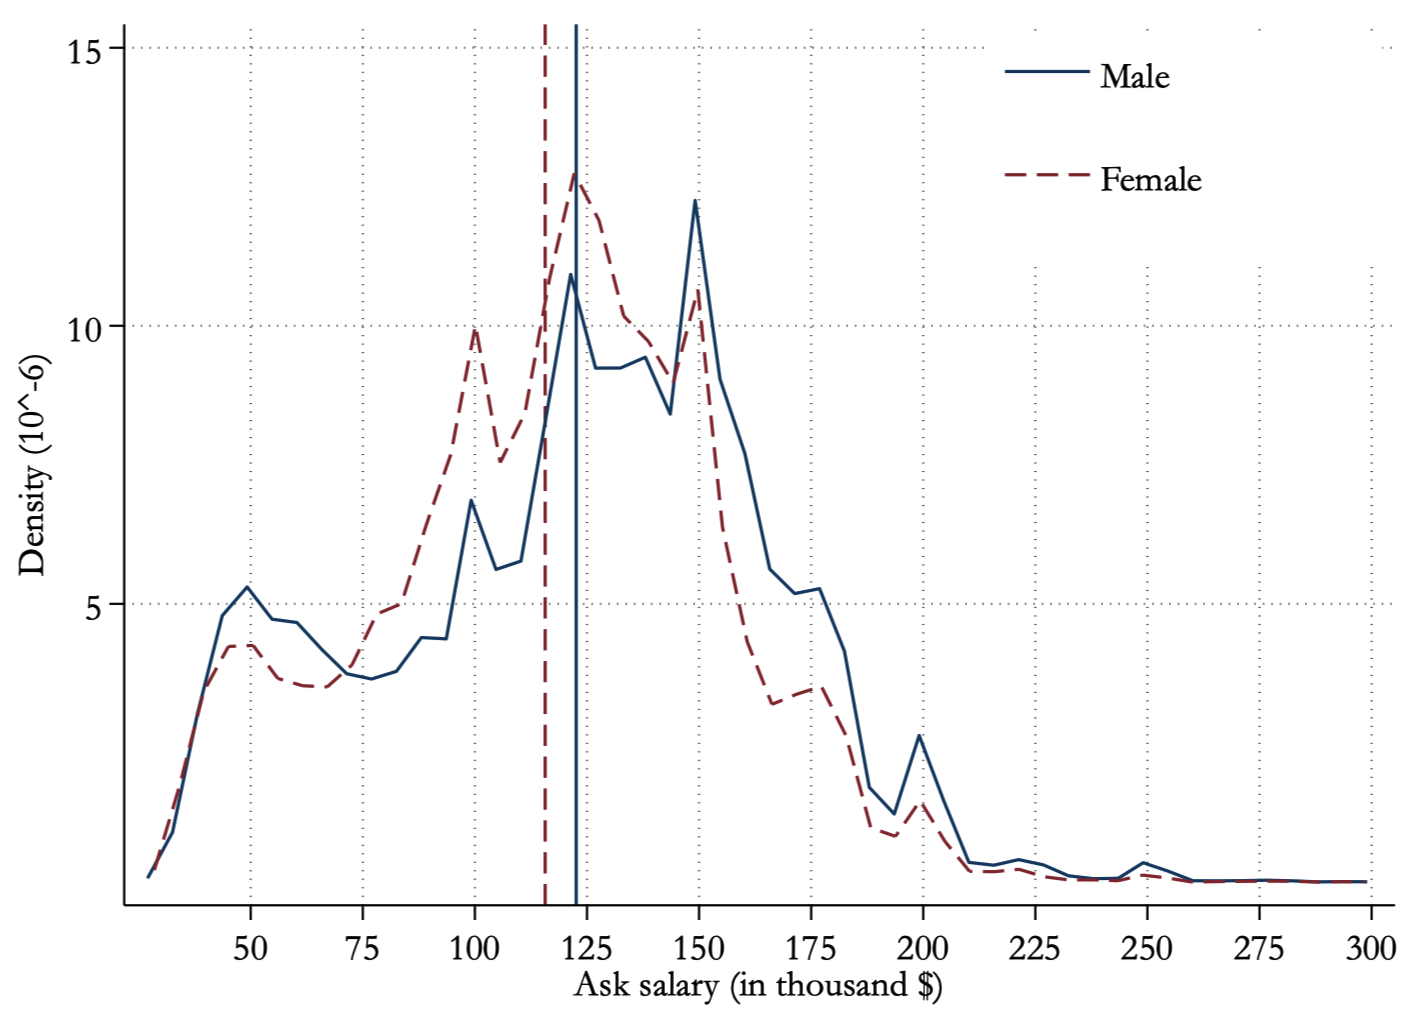
\includegraphics[height = 0.7 \textheight]{images/askgap.png}
       
        {\footnotesize \textcolor{frenchlilac!45!white}{\$ 115116} (female) - \textcolor{frenchlilac!45!white}{\$ 121942} (male) = \textcolor{frenchlilac!45!white}{-\$6826}}
    \end{figure}
\end{frame}

\begin{frame}{Ask Gap: Regression Results}
    $$ \log(Ask_{i\uncover<3>{b}}) = \alpha + \textcolor{frenchlilac!45!white}{\beta_0} Female_i \uncover<2->{+\beta_1 \mathbf{X}_{i\uncover<3>{b}}} + \gamma_t +\epsilon_{i\uncover<3>{b}} $$
    \vspace*{-10pt}
    \begin{table}[h!]
        \footnotesize
        \begin{center}
            \begin{tabular}{lccccc}
                \multicolumn{6}{l}{Dependent Variable: \textcolor{frenchlilac!45!white}{$\log(\text{Ask Salary})$}} \\
                \hline
                Female & \textcolor<1>{frenchlilac!45!white}{-0.068$^{***}$} & \textcolor<2>{frenchlilac!45!white}{-0.044$^{***}$} & \textcolor<2>{frenchlilac!45!white}{-0.029$^{***}$} & \textcolor<2>{frenchlilac!45!white}{-0.032$^{***}$} & \textcolor<3>{frenchlilac!45!white}{-0.024$^{***}$}\\
                \hline 
                Experience, city, occupation & & $\checkmark$ & $\checkmark$ & $\checkmark$& $\checkmark$\\
                Education, work preferences  & & $\checkmark$ & $\checkmark$ & $\checkmark$& $\checkmark$\\ 
                Employment history  & & & $\checkmark$ & $\checkmark$& $\checkmark$\\
                Firm (recent) FE  & & &  & $\checkmark$& \\
                Month $\times$ year FE &  $\checkmark$ & $\checkmark$& $\checkmark$ & $\checkmark$ & $\checkmark$ \\
                Adj. $R^2$ & 0.010 & 0.678 & 0.708 & 0.601 & 0.809 \\
                No. Obs & 113777 & 113777 & 113777 & 63916 & 463860 \\
            \end{tabular}
        \end{center}
    \end{table}
\end{frame}

\begin{frame}{Ask Gap: Heterogeneity}
    \begin{figure}
        \centering
        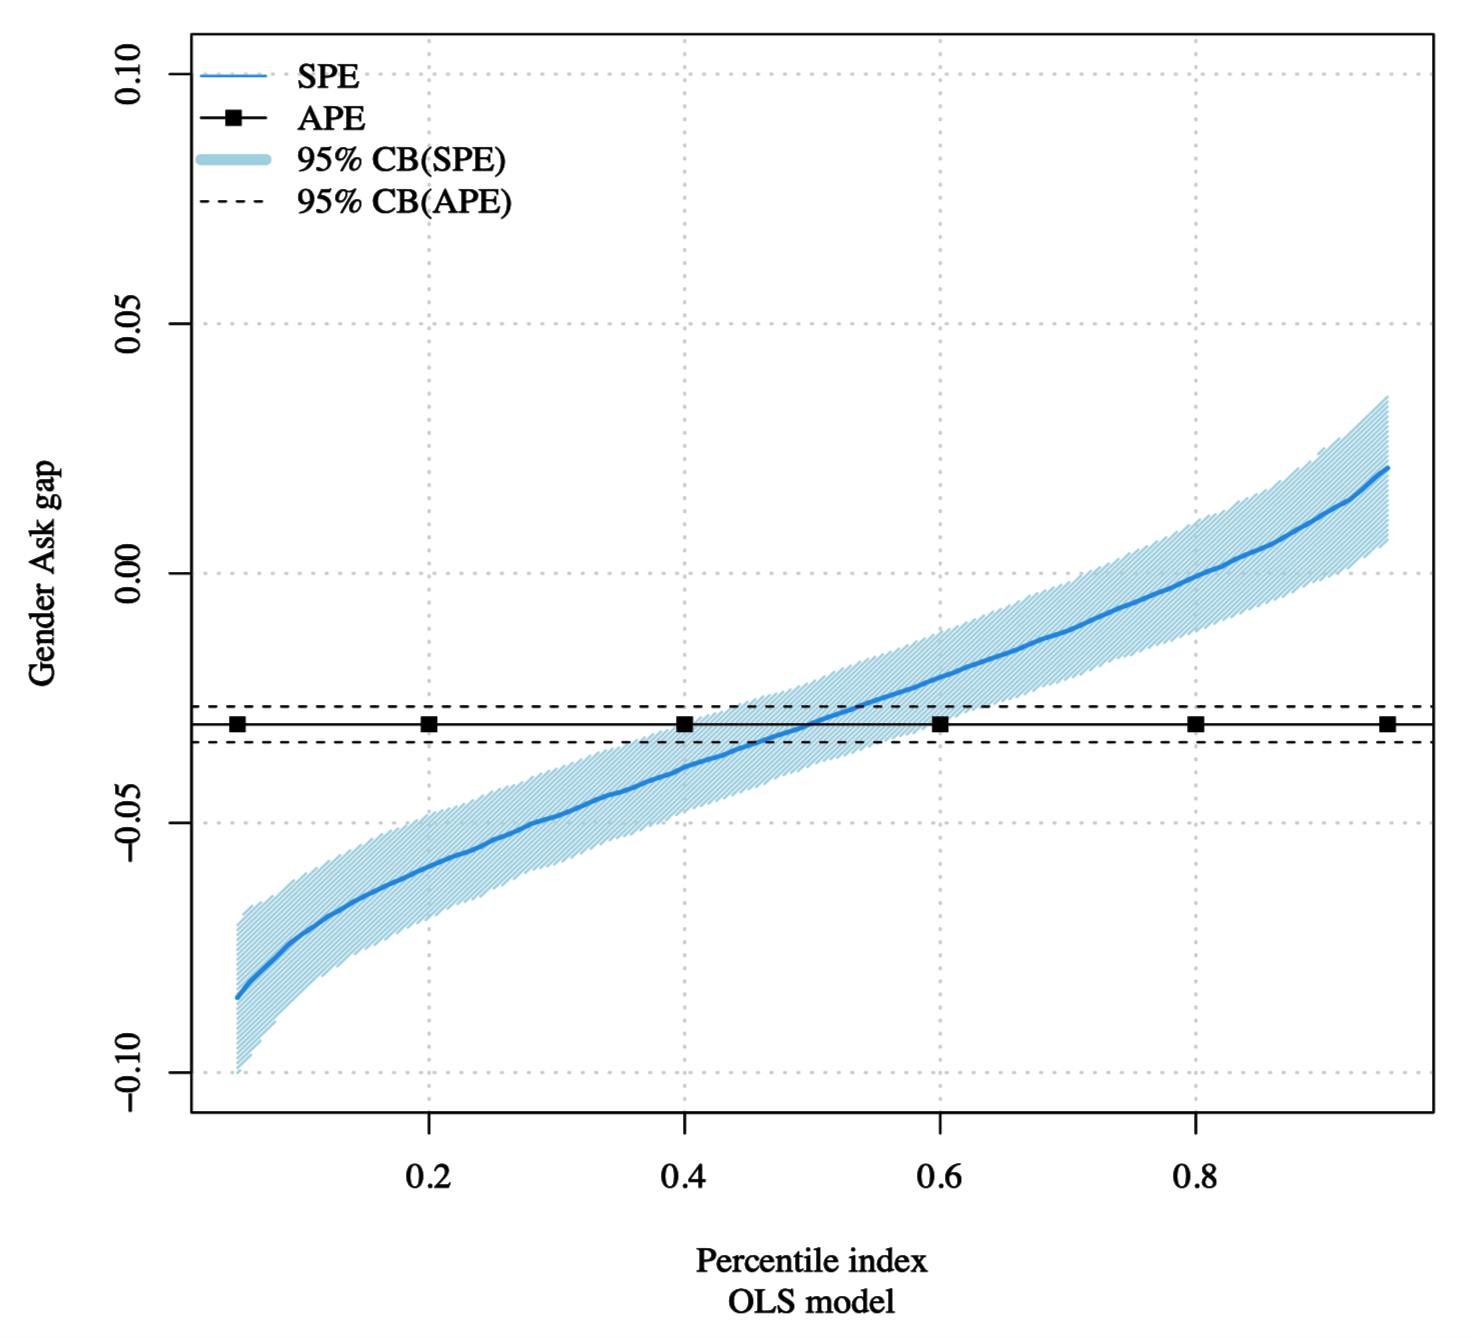
\includegraphics[height = 0.7 \textheight]{images/askgap_hetero.png}
       
        {\footnotesize Sorted Effects Method, following \citet{chernozhukov2018sorted}}
    \end{figure}
\end{frame}

\begin{frame}{Ask Gap: Heterogeneity by Experience}
    \begin{figure}
        \centering
        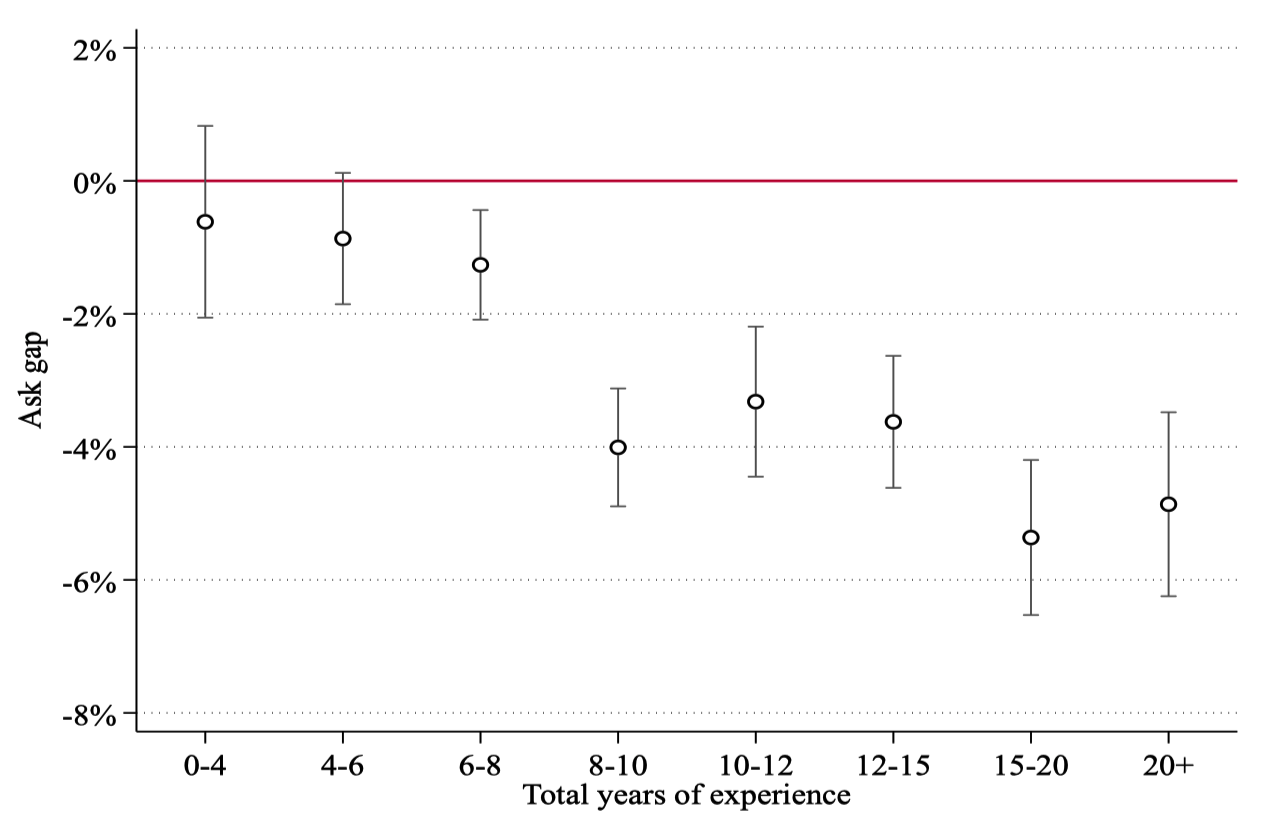
\includegraphics[height = 0.7 \textheight]{images/askgap_hetero_exp.png}
    \end{figure}
\end{frame}

\begin{frame}{Ask Gap: External Validity}
    \begin{table}[h!]
        \scriptsize
        \begin{center}
            \begin{tabular}{cccc}
                \hline
                \textcolor{frenchlilac!45!white}{\textit{Ask Gap: Raw}} \\
                { \citet{roussille2021central}} & {\tiny American Community Survey }& \\
                6.8\% & 8\% \\ \hline
                \textcolor{frenchlilac!45!white}{\textit{Ask Gap: Net}} \\
                { \citet{roussille2021central}} & {\tiny \citet{krueger2016contribut}} &{\tiny \citet{le2021gender}} & {\tiny Fluchtmann et al. (2021)}\\
                2.9\% & 8.3\% & 3.6\% & 1.9\% \\
                $R^2 = 0.71$ & & $R^2 = 0.73$ & \\
                \hline
            \end{tabular}
        \end{center}
    \end{table}
\end{frame}

\subsection*{Bid Gap}
\begin{frame}{Bid Gap: Graphic Evidence}
    \begin{figure}
        \centering
        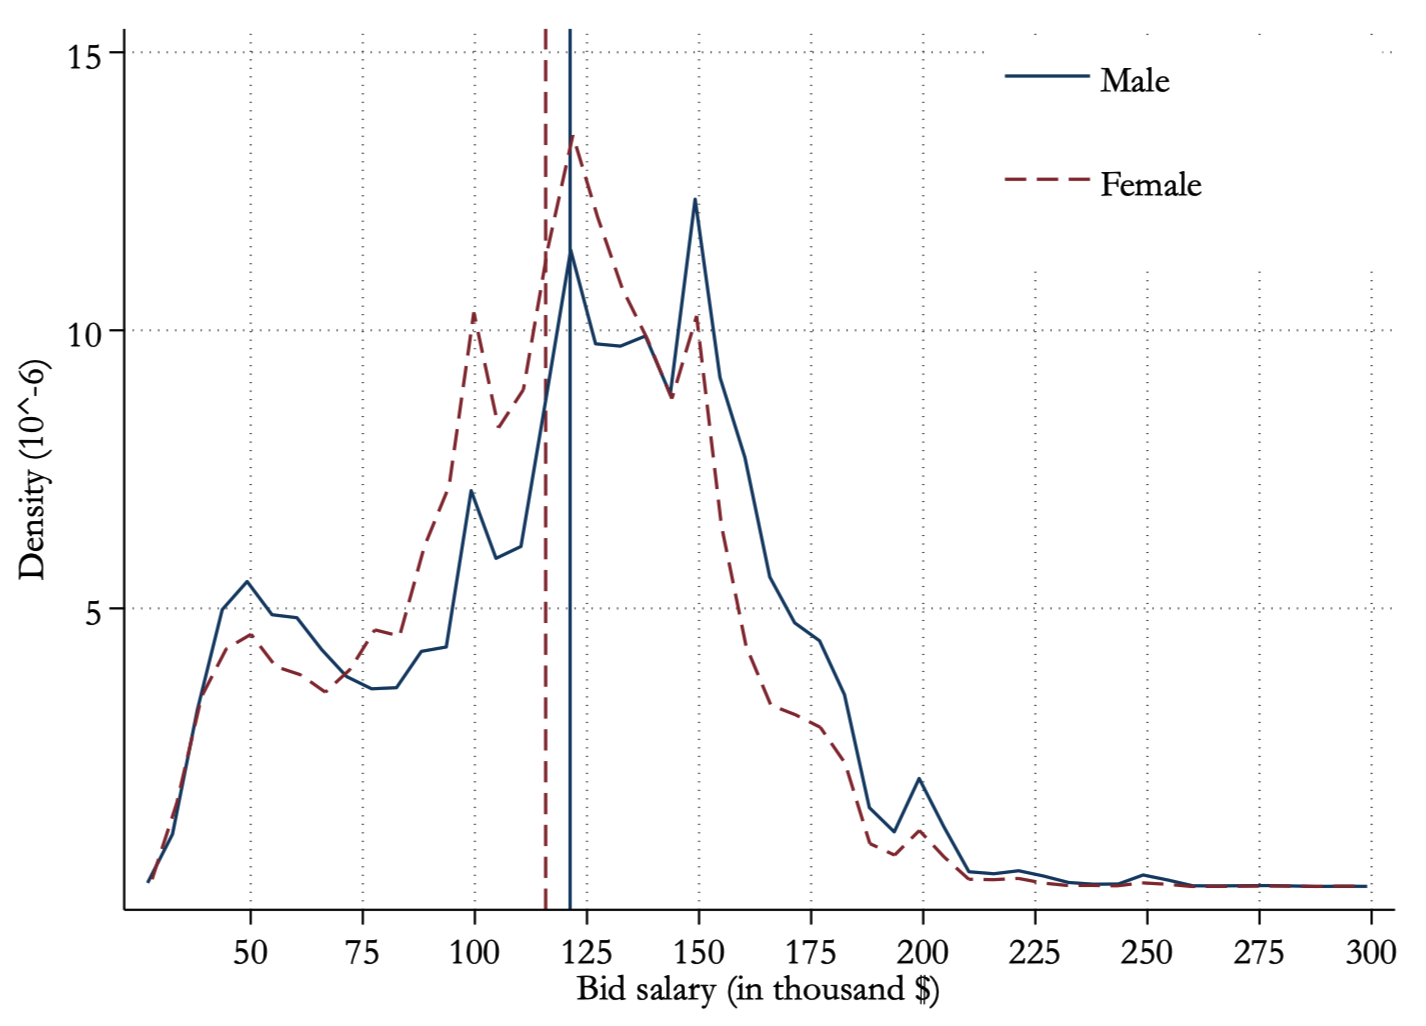
\includegraphics[height = 0.7 \textheight]{images/bidgap.png}
        
        {\footnotesize \textcolor{frenchlilac!45!white}{\$ 115290} (female) - \textcolor{frenchlilac!45!white}{\$ 120720} (male) = \textcolor{frenchlilac!45!white}{-\$5430}}
    \end{figure}
\end{frame}

\begin{frame}{Bid Gap: Regression Results}
    
    {\footnotesize
     $$ \log(Bid_{ib}) = \alpha + \textcolor{frenchlilac!45!white}{\beta_1} Female_i \only<2,4-5>{+\beta_2 \mathbf{X}_{ib}} + \gamma_t \only<3->{+ \beta_3 \log(Ask_{ib})} \only<5>{+ \textcolor{frenchlilac!45!white}{\beta_4} \log(Ask_{ib}\times Female_i)} +\epsilon_{ib} $$}
    \vspace*{-10pt}
    \begin{table}[h!]
        \footnotesize
        \begin{center}
            \begin{tabular}{lccccc}
                \multicolumn{6}{l}{Dependent Variable: \textcolor{frenchlilac!45!white}{$\log(\text{Bid Salary})$}} \\
                \hline
                Female & \textcolor<1>{frenchlilac!45!white}{-0.034$^{***}$} & \textcolor<2>{frenchlilac!45!white}{-0.022$^{***}$} & \textcolor<3>{frenchlilac!45!white}{0.002$^{***}$} & \textcolor<4>{frenchlilac!45!white}{-0.002$^{***}$} & \textcolor<5>{frenchlilac!45!white}{-0.002$^{***}$}\\
                $\log(\text{Ask Salary})$ & & & {0.963$^{***}$} & {0.849$^{***}$} & {0.848$^{***}$} \\
                Female $\times \log(\text{Ask Salary})$  & & & & &  \textcolor<5>{frenchlilac!45!white}{0.001}\\
                \hline 
                Resume characteristics & & $\checkmark$ & & $\checkmark$& $\checkmark$\\
                Month $\times$ year FE &  $\checkmark$ & $\checkmark$& $\checkmark$ & $\checkmark$ & $\checkmark$ \\
                Adj. $R^2$ & 0.007 & 0.816 & 0.950 & 0.954 & 0.954 \\
                No. Obs & 463860 & 463860 & 463860 & 463860 & 463860 \\
            \end{tabular}
        \end{center}
    \end{table}
\end{frame}

\begin{frame}{Bid Gap: Within-Job Regression Results}
    
    \begin{table}[h!]
        \footnotesize
        \begin{center}
            \begin{tabular}{lccccc}
                \multicolumn{6}{l}{Dependent Variable: \textcolor{frenchlilac!45!white}{$\log(\text{Bid Salary})$}} \\
                \hline
                Female & \textcolor{frenchlilac!45!white}{-0.049$^{***}$} & \textcolor{frenchlilac!45!white}{-0.018$^{***}$} & \textcolor{frenchlilac!45!white}{-0.006$^{***}$} & \textcolor{frenchlilac!45!white}{-0.003$^{***}$} & \textcolor{frenchlilac!45!white}{-0.003$^{***}$}\\
                \uncover<2>{{\tiny no job FE} & {\tiny -0.034$^{***}$} & {\tiny -0.022$^{***}$} & {\tiny 0.002$^{***}$} & {\tiny -0.002$^{***}$} & {\tiny -0.002$^{***}$}\\}
                $\log(\text{Ask Salary})$ & & & {0.963$^{***}$} & {0.849$^{***}$} & {0.848$^{***}$} \\
                \uncover<2>{{\tiny no job FE} & & & {\tiny 0.805$^{***}$} & {\tiny 0.774$^{***}$} & {\tiny 0.774$^{***}$}} \\
                Female $\times \log(\text{Ask Salary})$  & & & & &  \textcolor{frenchlilac!45!white}{0.001}\\
                \uncover<2>{{\tiny no job FE} & & & & & {\tiny 0.003}}\\
                \hline 
                Resume characteristics & & $\checkmark$ & & $\checkmark$& $\checkmark$\\
                \textcolor{frenchlilac!45!white}{Job FE} &  $\checkmark$ & $\checkmark$& $\checkmark$ & $\checkmark$ & $\checkmark$ \\
                Month $\times$ year FE &  $\checkmark$ & $\checkmark$& $\checkmark$ & $\checkmark$ & $\checkmark$ \\
                Adj. $R^2$ & 0.014 & 0.329 & 0.828 & 0.834 & 0.834 \\
                \uncover<2>{{\tiny no job FE} & {\tiny 0.007} & {\tiny 0.816} & {\tiny 0.950} & {\tiny 0.954} & {\tiny 0.954}} \\
                No. Obs & 454631 & 454631 & 454631 & 454631 & 454631 \\
            \end{tabular}
        \end{center}
    \end{table}
\end{frame}

\begin{frame}{Bid Gap: Heterogeneity by Experience}

    \begin{columns}[T]
        \begin{column}{0.45\textwidth}
            \begin{figure}
                \centering
                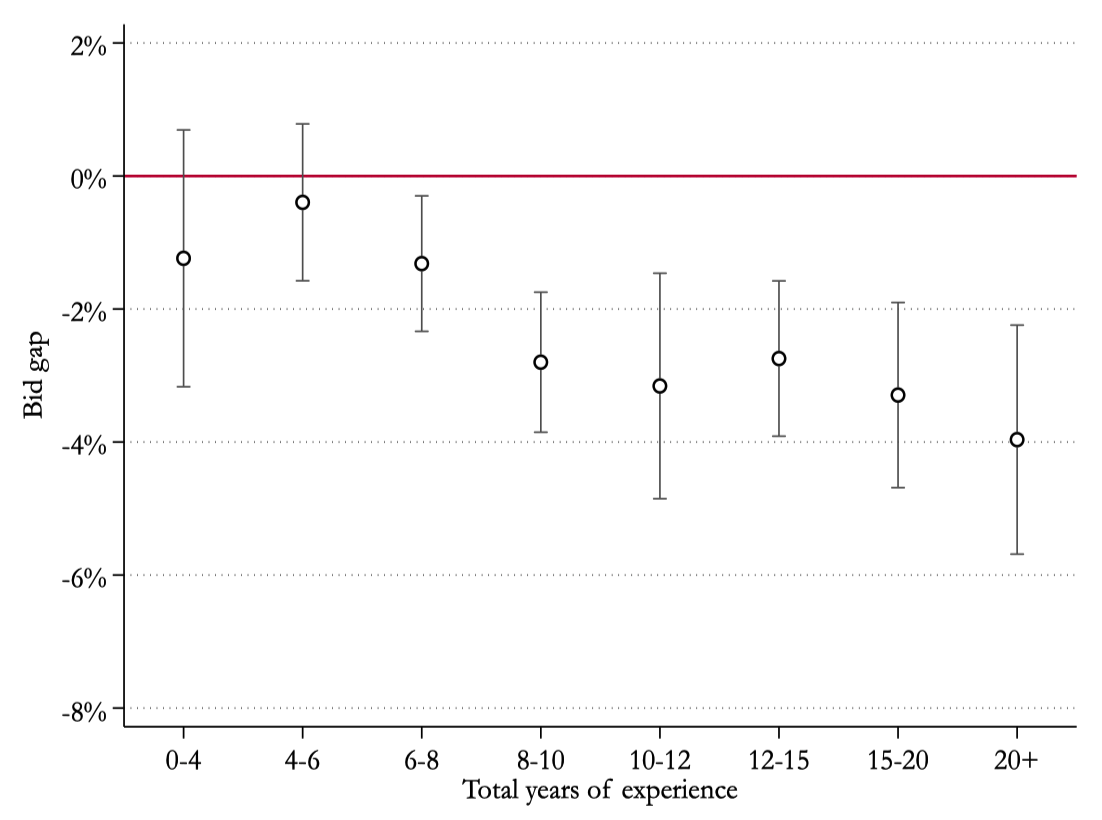
\includegraphics[height = 0.57 \textheight]{images/bidgap_hetero_exp.png}
                
                {\footnotesize Bid gap by experience}
            \end{figure}
        \end{column}

        \begin{column}{0.45\textwidth}
            \begin{figure}
                \centering
                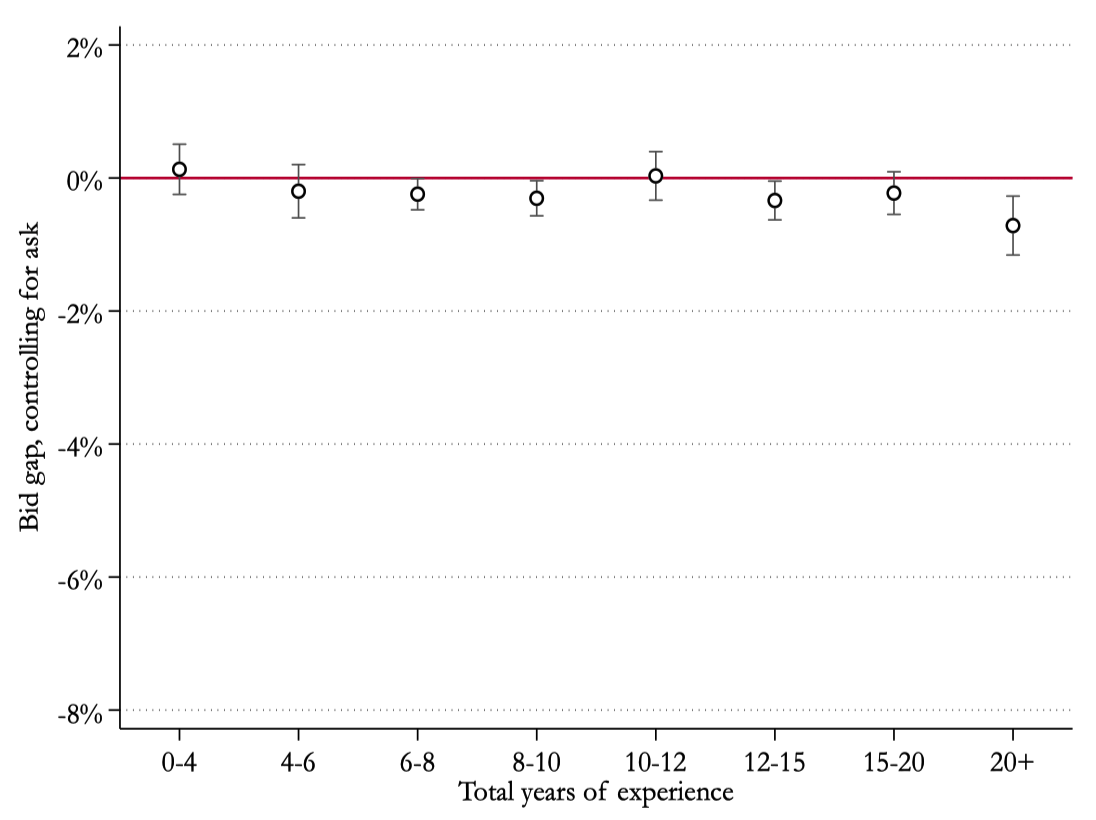
\includegraphics[height = 0.57 \textheight]{images/bidgap_hetero_exp_gender.png}
                
                {\footnotesize Bid gap by experience, net of Ask gap}
            \end{figure}
        \end{column}
    \end{columns}
    
\end{frame}

\begin{frame}{Bid Gap: External Validity}
    \begin{table}[h!]
        \scriptsize
        \begin{center}
            \begin{tabular}{cccc}
                \hline
                \textcolor{frenchlilac!45!white}{\textit{Ask Gap: Net}} \\
                { \citet{roussille2021central}} & { \citet{blau2017gender}} &{ Chamberlain et al. (2019)} \\
                2.2\% & 8.4\% & 5.4\%  \\
                & { Fluchtmann et al. (2021)} & { \citet{le2021gender}} \\
                & 1.9\% & 3.7\% \\
                \hline
            \end{tabular}
        \end{center}
    \end{table}
\end{frame}

\subsection*{Final Gap}

\begin{frame}{Final Gap: Regression Results}
    
    \begin{table}[h!]
        \scriptsize
        \begin{center}
            \begin{tabular}{lccccc}
                \multicolumn{6}{l}{Dependent Variable: \textcolor{frenchlilac!45!white}{$\log(\text{Final Salary})$}} \\
                \hline
                Female & \textcolor{frenchlilac!45!white}{-0.049$^{***}$} & \textcolor{frenchlilac!45!white}{-0.014$^{***}$} & \textcolor{frenchlilac!45!white}{0.023$^{***}$} & \textcolor{frenchlilac!45!white}{0.009$^{***}$} & \textcolor{frenchlilac!45!white}{0.010$^{***}$}\\
                $\log(\text{Ask Salary})$ & & & {0.956$^{***}$} & {0.712$^{***}$} & {0.709$^{***}$} \\
                Female $\times \log(\text{Ask Salary})$  & & & & &  \textcolor{frenchlilac!45!white}{0.011}\\
                \hline 
                Resume characteristics & & $\checkmark$ & & $\checkmark$& $\checkmark$\\
                Adj. $R^2$ & 0.012 & 0.827 & 0.903 & 0.920 & 0.920 \\
                No. Obs & 7582 & 7582 & 7582 & 7582 & 7582 \\
                & \\ \hline\hline 
                & \\
                Female & & \textcolor{frenchlilac!45!white}{-0.018$^{***}$} &  & \textcolor{frenchlilac!45!white}{0.002} & \textcolor{frenchlilac!45!white}{0.003}\\
                $\log(\text{Ask Salary})$ & & &  & {0.617$^{***}$} & {0.615$^{***}$} \\
                Female $\times \log(\text{Ask Salary})$  & & & & &  \textcolor{frenchlilac!45!white}{0.008}\\
                \hline 
                Resume characteristics & & $\checkmark$ & & $\checkmark$& $\checkmark$\\
                \textcolor{frenchlilac!45!white}{Firm FE} & &$\checkmark$ &  & $\checkmark$ & $\checkmark$ \\
                Adj. $R^2$ & & 0.515 & & 0.762 & 0.762 \\
                No. Obs & & 6303 & & 6303 & 6303 \\

            \end{tabular}
        \end{center}
    \end{table}
\end{frame}

\begin{frame}{A Summary of Robustness Check}
    \begin{itemize}
        \item<+-> Explanation power of Ask Salary
        \begin{itemize}
            \footnotesize
            \item Bid Salary: reducing the prediction power of experience and education
            \item Final Salary: eliminating the prediction power of education, reducing that of experience to $\sim$ 0
        \end{itemize}
        \item<+-> Compensation structure: adding equity offers does \textcolor{frenchlilac!45!white}{\textit{NOT}} change the results
        \item<+-> Firm selection
        \begin{itemize}
            \footnotesize
            \item Search effort: firms that end up hiring are \textcolor{frenchlilac!45!white}{\textit{NOT}} different from the full sample 
            \item Pricing effort: gender gap results are \textcolor{frenchlilac!45!white}{\textit{robust}} for firms that do not take ask prices as bid prices
        \end{itemize}
        \item<+-> Candidates
        \begin{itemize}
            \footnotesize
            \item Selective updating: adding spell FEs does \textcolor{frenchlilac!45!white}{\textit{NOT}} change the results;  an interesting \textcolor{frenchlilac!45!white}{\textit{asymmetry}} of updating: upward updating benefits more
            \item Racial gap: similar results for racial minority groups' negotiations
        \end{itemize}
    \end{itemize}
\end{frame}

\subsection*{Extensive Margin}

\begin{frame}{Extensive Margin: Selection for Interview}
    \begin{table}[h!]
        \scriptsize
        \begin{center}
            \begin{tabular}{lccccc}
                \multicolumn{6}{l}{Dependent Variable: \textcolor{frenchlilac!45!white}{Number of bids received}} \\
                \hline
                Female & {-0.397$^{***}$} & \textcolor{frenchlilac!45!white}{0.227$^{***}$} & \textcolor{frenchlilac!45!white}{0.259$^{***}$} & \textcolor{frenchlilac!45!white}{0.271$^{***}$} & \textcolor{frenchlilac!45!white}{0.342$^{***}$}\\
                $\text{Ask Salary}$ & & & {0.937$^{***}$} & {1.924$^{***}$} & {0.979$^{***}$} \\
                $\text{Ask Salary}^2$ & & & & {-0.228$^{***}$} &  \\
                Female $\times (\text{Ask Salary})$  & & & & &  {-0.074}\\
                \hline 
                Poisson AME on Female & -0.402 & 0.303 & 0.329 & 0.361 & 0.326 \\
                Resume characteristics & & $\checkmark$ & $\checkmark$ & $\checkmark$& $\checkmark$\\
                Adj. $R^2$ & 0.015 & 0.240 & 0.244 & 0.245 & 0.244 \\
                No. Obs & 164799 & 164799 & 164799 & 164799 & 164799 
            \end{tabular}
        \end{center}
    \end{table}
\end{frame}

\begin{frame}{Extensive Margin: Selection for Interview}
    \begin{figure}
        \centering
        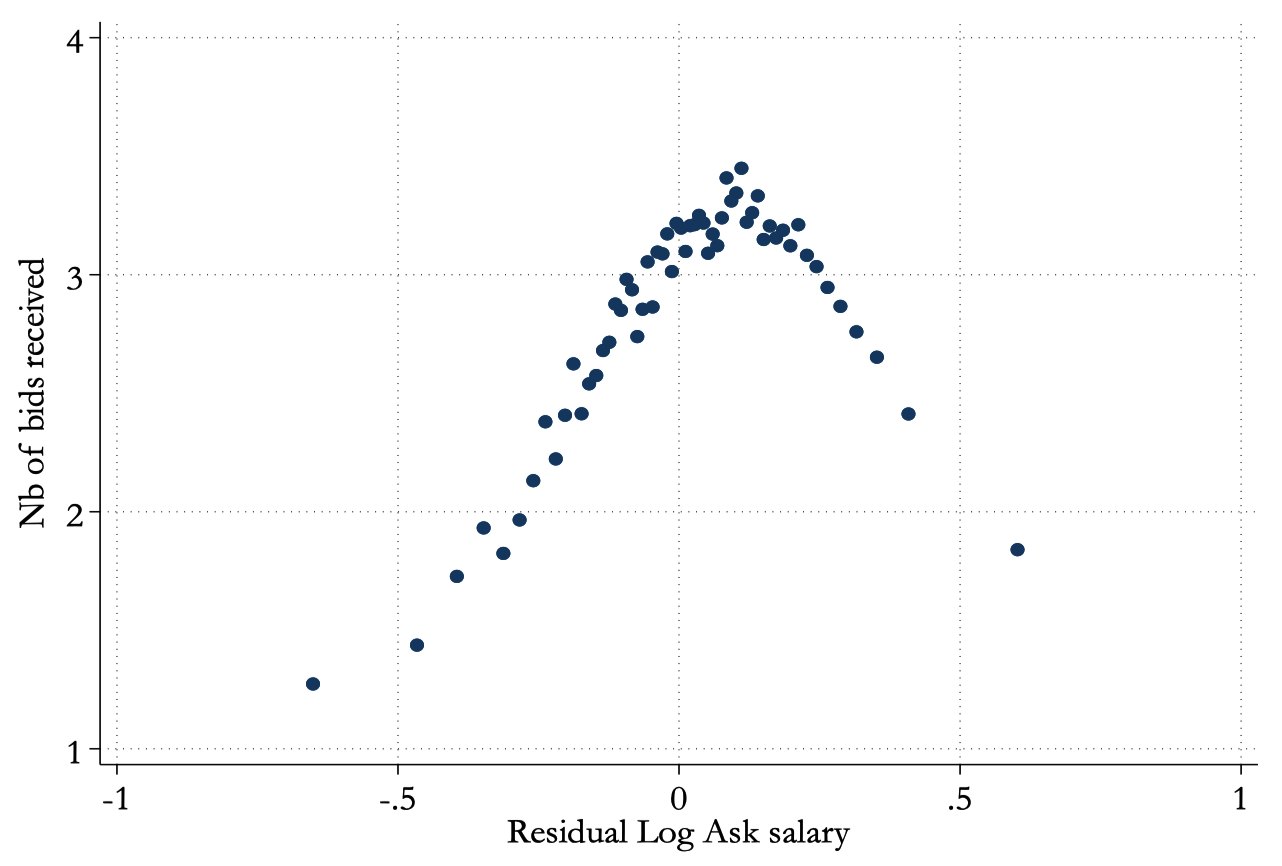
\includegraphics[height = 0.7 \textheight]{images/ask_nobids.png}
    \end{figure}
\end{frame}

\begin{frame}{Extensive Margin: Receiving A Final Offer After Interview}
    \begin{table}[h!]
        \scriptsize
        \begin{center}
            \begin{tabular}{lcccc}
                \multicolumn{5}{l}{Dependent Variable: \textcolor{frenchlilac!45!white}{$\Pr(\text{Final offer received after interview})$}} \\
                \hline
                Female & 0.001 & 0.001 & 0.001 &-0.000\\
                $\text{Ask Salary}$ & & & -0.000& 0.023$^{***}$ \\
                $\text{Ask Salary}^2$ & & & 0.001 & {-0.002$^{***}$} \\
                \hline 
                Logit AME on Female & 0.001 & 0.000 & 0.000 & -0.018\\
                Resume characteristics & & $\checkmark$ & $\checkmark$ & $\checkmark$ \\
                Job FE & & & & $\checkmark$ \\
                Adj. $R^2$ & 0.000 & 0.008 & 0.008 & 0.006 \\
                No. Obs & 261518 & 261518 & 261518 & 251817 
            \end{tabular}
        \end{center}
    \end{table}
\end{frame}

\begin{frame}{Extensive Margin: Quality of Job Search}
    
    {\footnotesize
    \begin{itemize}
        \item<1-> \underline{\textit{Ranking by bids}}: $j$ is ranked above $k$ if they bid at the same salary, but candidate $i$ choose $j$ over $k$
        \item<3-> \underline{\textit{Ranking by offers}}: $j$ is ranked above $k$ if they offer the same salary, but candidate $i$ accept $j$ over $k$
    \end{itemize}
    }
    
    \uncover<2->{
        \begin{table}[h!]
            \scriptsize
            \begin{center}
                \begin{tabular}{lcccccc}
                    Dep. Var. & \multicolumn{3}{c}{\textcolor{frenchlilac!45!white}{Firm rank (by \textit{bid})}} & \multicolumn{3}{c}{ \uncover<3->{\textcolor{frenchlilac!45!white}{Firm rank (by \textit{offer})}} }  \\ \hline
                    Female & {-1.795$^{***}$} & \textcolor{frenchlilac!45!white}{-0.042} & \textcolor{frenchlilac!45!white}{0.163} & \uncover<3->{-1.241 & \textcolor{frenchlilac!45!white}{0.856} & \textcolor{frenchlilac!45!white}{1.254}} \\
                    $\log(\text{Ask Salary})$ & & & \textcolor{frenchlilac!45!white}{8.785$^{***}$} & & & \uncover<3->{\textcolor{frenchlilac!45!white}{13.157$^{***}$}} \\
                    \hline 
                    Resume characteristics & & $\checkmark$ & $\checkmark$ & & \uncover<3->{$\checkmark$ & $\checkmark$} \\
                    Mean rank percentile & 62.5 & 62.5 & 62.5 & \uncover<3->{64.3 & 64.3 & 64.3}\\
                    Adj. $R^2$ & 0.004 & 0.042 & 0.045 & \uncover<3->{0.005 & 0.088 & 0.096}  \\
                    No. Obs & 259749 & 259749 & 259749 & \uncover<3->{3454 & 3454 & 3454}
                \end{tabular}
            \end{center}
        \end{table}
    }
\end{frame}

\begin{frame}{Extensive Margin: Quality of Job Search}
    \begin{figure}
        \centering
        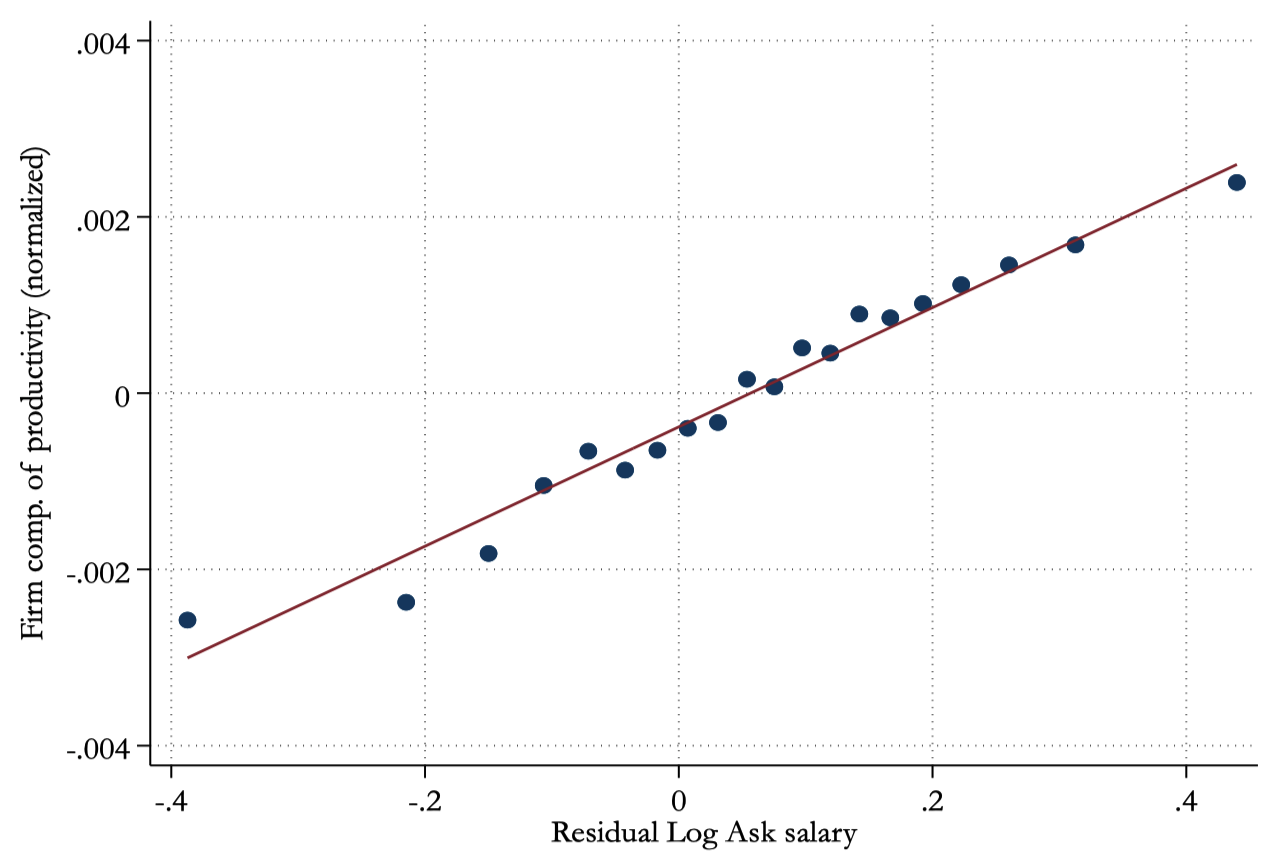
\includegraphics[height = 0.7 \textheight]{images/ask_productivity.png}

        {\footnotesize Expected match productivity inferred from firms' bids}
    \end{figure}
\end{frame}

\begin{frame}{The Model: Firm-Side Intuition}
    \begin{figure}
        \centering
        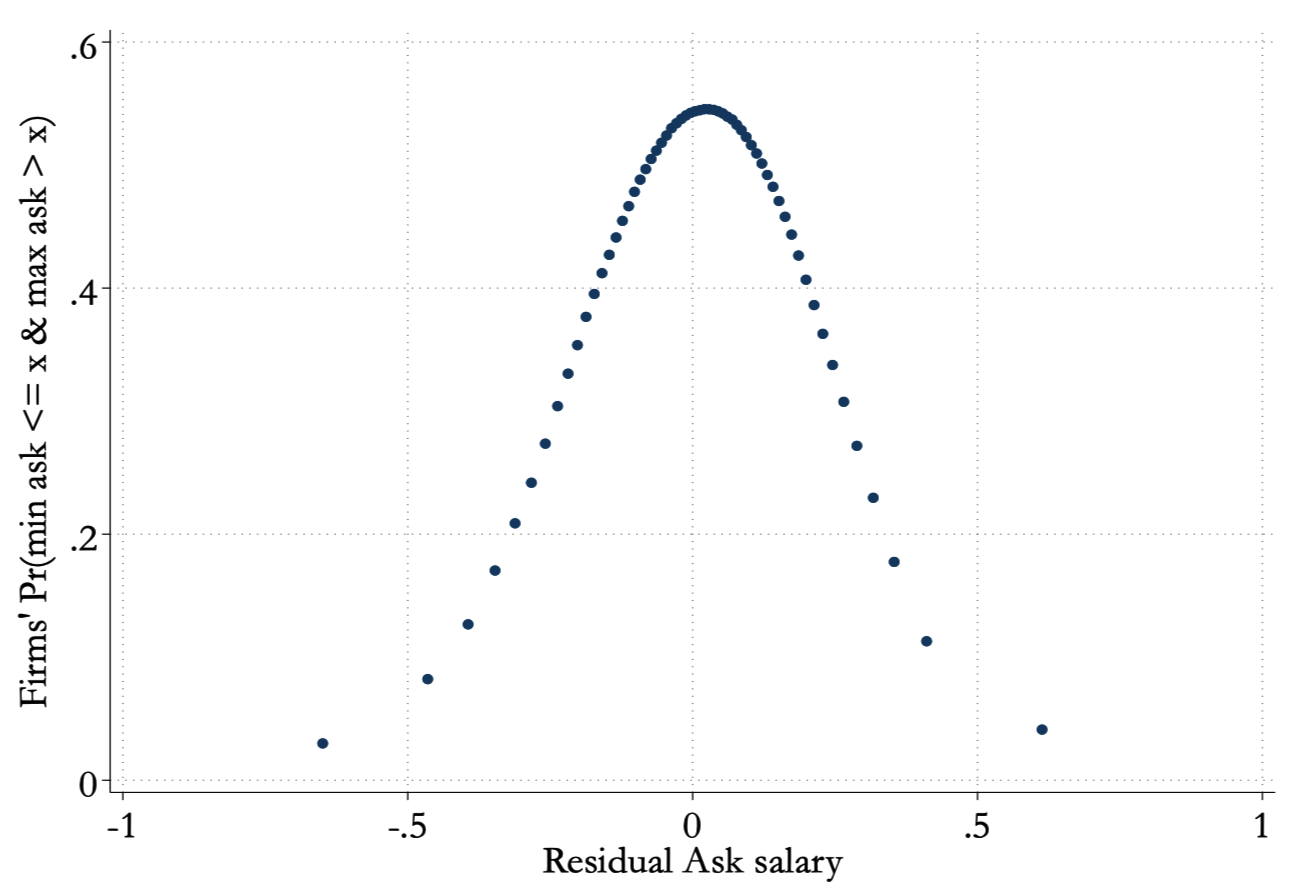
\includegraphics[height = 0.7 \textheight]{images/model_intuit.png}

        {\footnotesize Range of residual ask salaries that firms interview in}
    \end{figure}
\end{frame}

\subsection*{A Signal Model}
\begin{frame}{The Model: Gender Gap Persists with Ask Salary as Signal}
    \begin{center}
        \begin{tikzpicture}[every node/.append style={font=\small}]
            % Draw the axes
            \draw [white, very thick] (-6,0) -- (6,0) node[right]{wage};
            \draw [->, very thick, color = frenchlilac!45!white] (0,1.5) node[above]{$\text{salary}_{\text{ask}}$} -- (0,0);

            {\draw [white, very thick] (4.5,0) -- (4.5,0.2);
            \draw [white, very thick] (0.5,0) -- (0.5,0.2);
            \draw[decorate,decoration={brace,amplitude=5pt,raise=5pt},yshift=0pt, very thick, color=frenchlilac!45!white] (0.5,0) -- (4.5,0) node [midway, yshift=15pt, xshift =0pt]{\textit{over-qualified}};}
            
            {\draw [white, very thick] (-4.5,0) -- (-4.5,0.2);
            \draw [white, very thick] (-0.5,0) -- (-0.5,0.2);
            \draw[decorate,decoration={brace,amplitude=5pt,raise=5pt},yshift=0pt, very thick, color=frenchlilac!45!white] (-4.5,0) -- (-0.5,0) node [midway, yshift=15pt, xshift =0pt]{\textit{under-qualified}};}

            {
            \draw [white, very thick] (2,-0.2) -- (2,0);
            \draw [white, very thick] (-2,-0.2) -- (-2,0);
            \draw[decorate,decoration={brace,amplitude=5pt,raise=5pt,mirror},yshift=0pt, very thick, color=frenchlilac!45!white] (-2,0) -- (2,0) node [midway, yshift=-15pt, xshift =0pt]{\textit{rightfully qualified}};
            }

            \uncover<2->{\draw [citrine, very thick, densely dashed] (-0.5,0) -- (-0.5,0.75);
                \draw [citrine, very thick, densely dashed] (3.5,0) -- (3.5,0.75);
                \draw[decorate,decoration={brace,amplitude=5pt,raise=22pt},yshift=0pt, very thick, densely dashed, color=citrine] (-0.5,0) -- (3.5,0) node [midway, yshift=32pt, xshift =45pt]{\textit{over-qualified but under-asking: female}};}

        % Done
        \end{tikzpicture}
    \end{center}
\end{frame}

\subsection*{Closing the Gap}
\begin{frame}{An Information Treatment}
    \begin{figure}
        \centering
        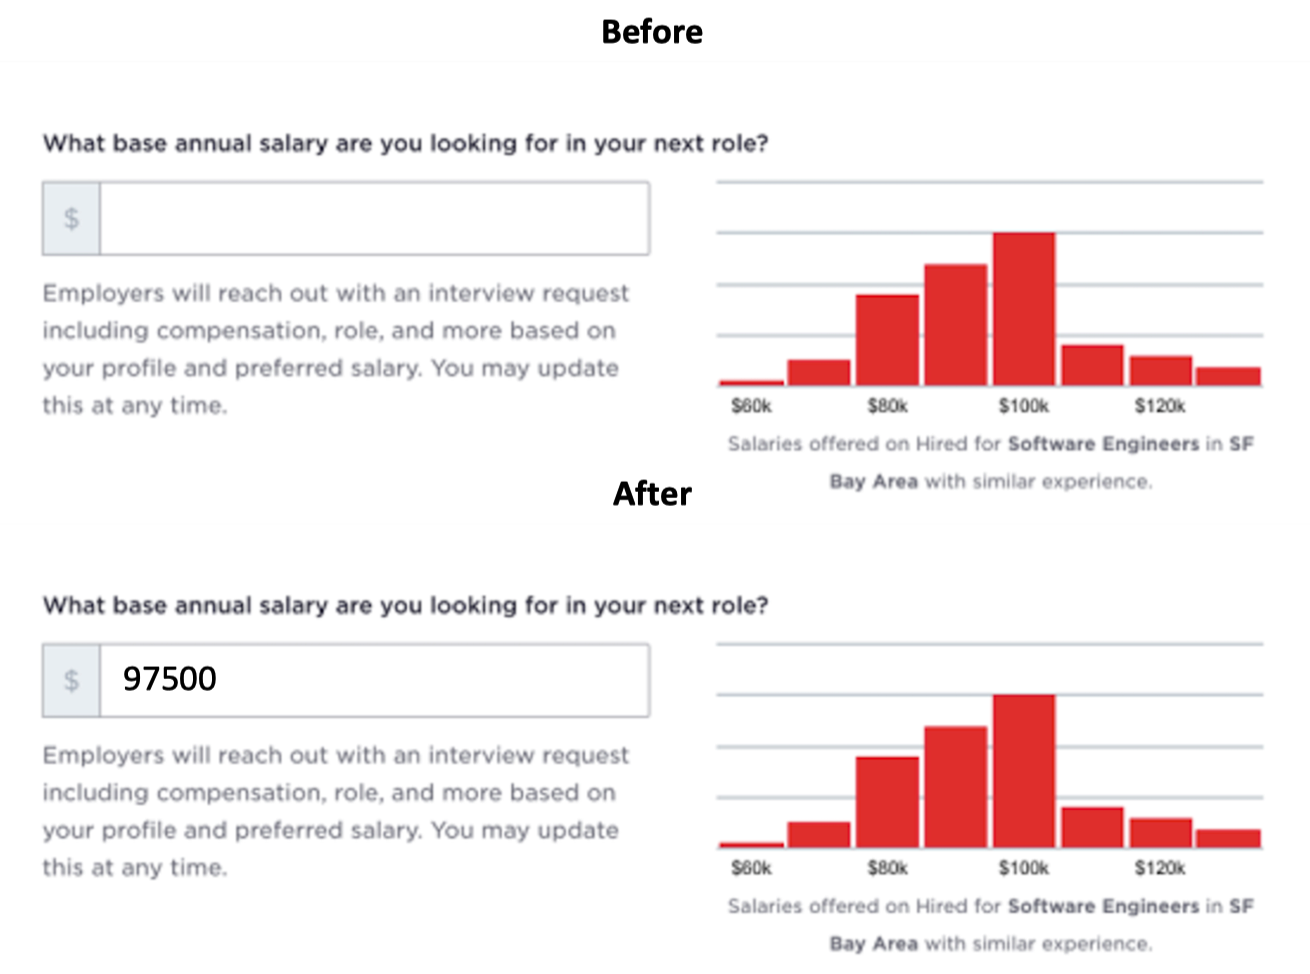
\includegraphics[height = 0.75 \textheight]{images/treat.png}
    \end{figure}
\end{frame}

\begin{frame}{Treatment Effect: Ask Gap}
    \begin{columns}
        \begin{column}{0.6\textwidth}
            \begin{figure}
                \centering
                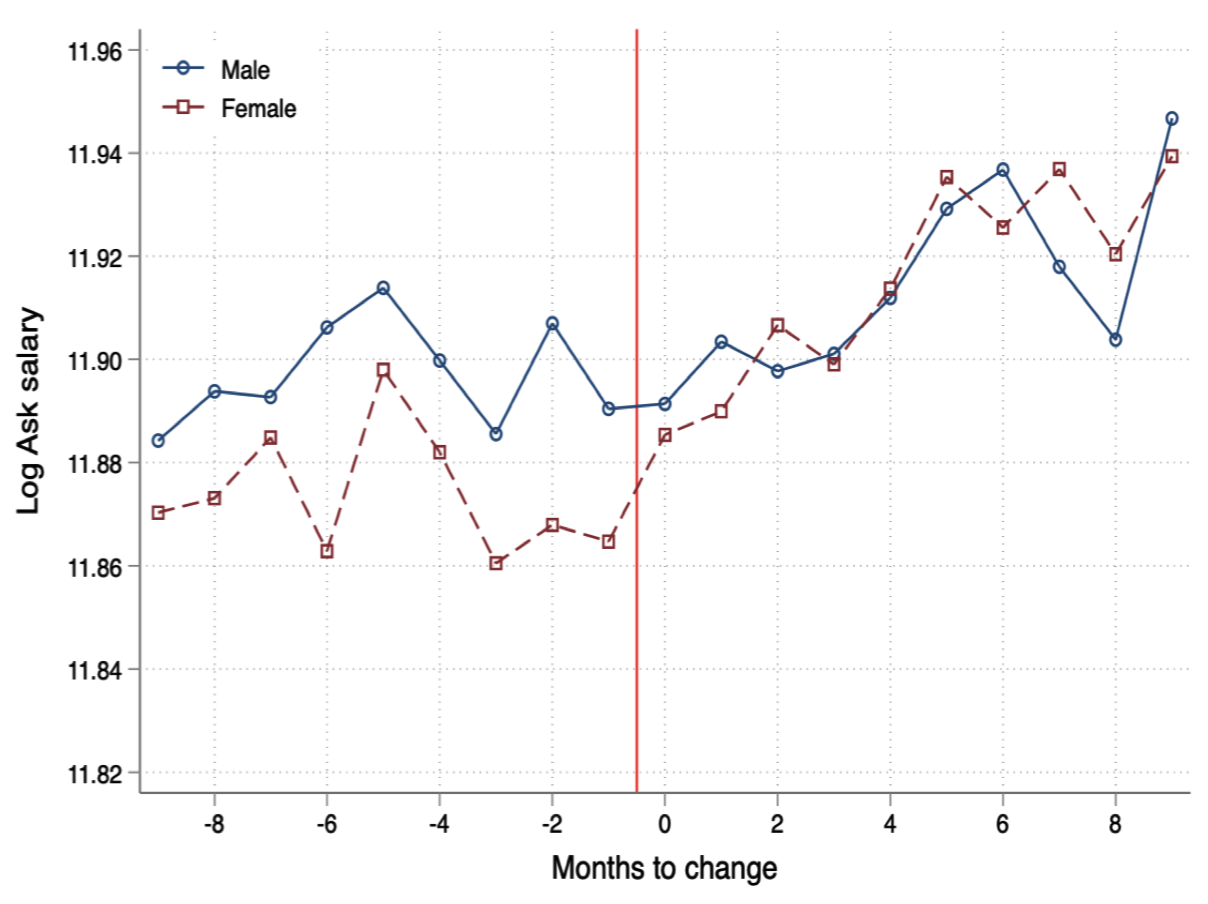
\includegraphics[width = 0.9 \textwidth]{images/treat_ask.png}
            \end{figure}
        \end{column}

        \begin{column}{0.4\textwidth}
            \begin{table}[h!]
                \scriptsize
                \begin{center}
                    \begin{tabular}{lc}
                        \multicolumn{2}{c}{Placebo} \\
                         & Ask Gap  \\
                         & predicted \\ \hline
                        Female & -0.080$^{***}$ \\
                        After & 0.002 \\
                        Female $\times$ After & -0.003\\
                        \hline 
                        Adj. $R^2$ & 0.02  \\
                        No. Obs & 43368
                    \end{tabular}
                \end{center}
            \end{table}
        \end{column}
    \end{columns}
\end{frame}

\begin{frame}{Treatment Effect: Bid Gap}
    \begin{figure}
        \centering
        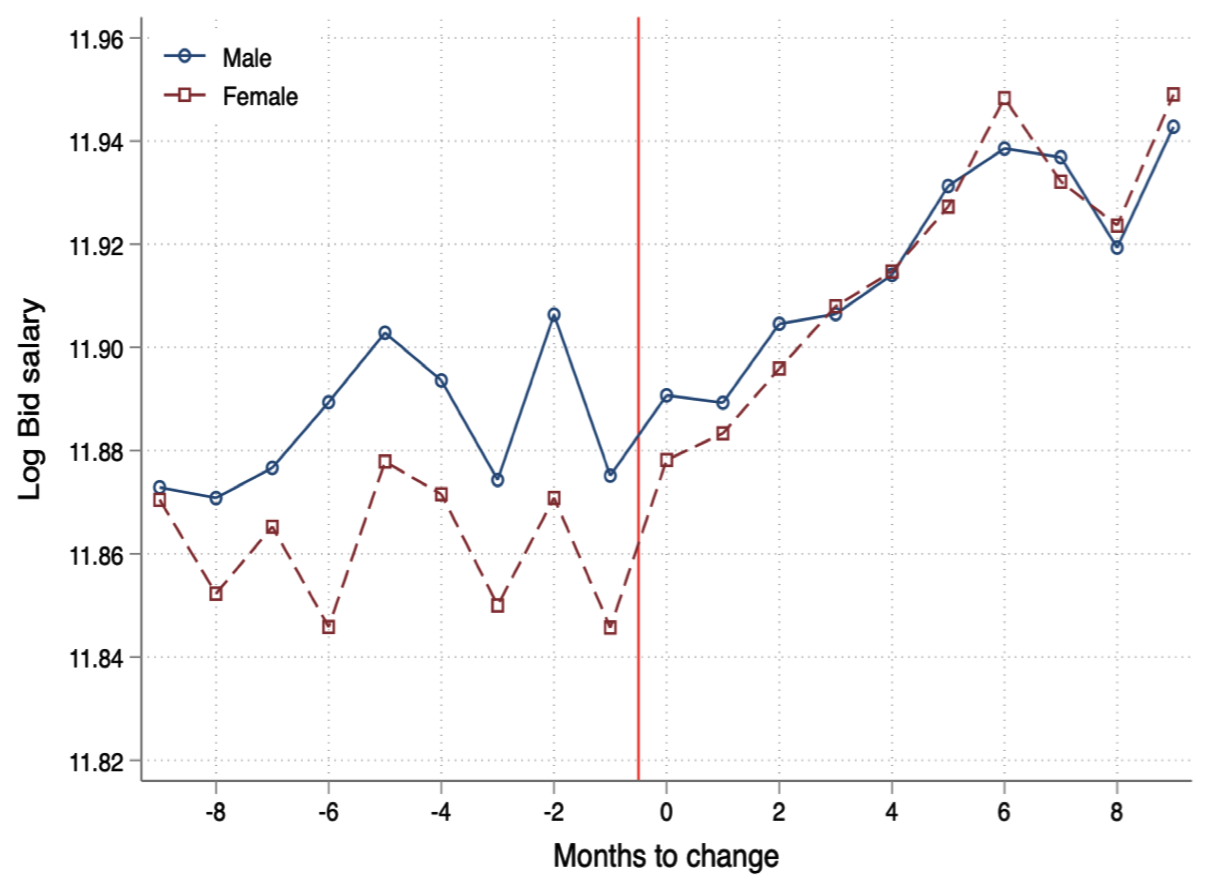
\includegraphics[height = 0.75 \textheight]{images/treat_bid.png}
    \end{figure}
\end{frame}

\begin{frame}{Treatment Effect: Final Gap}
    \begin{figure}
        \centering
        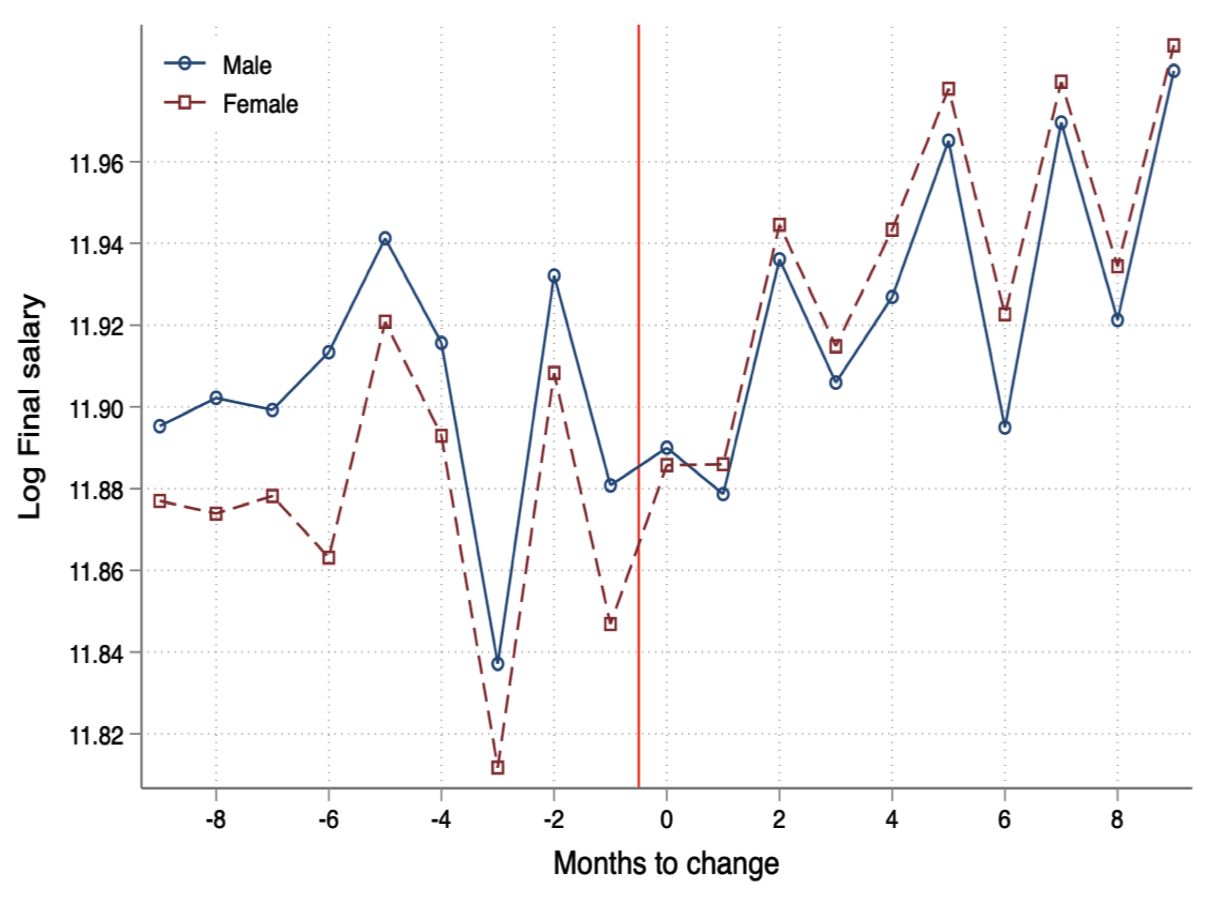
\includegraphics[height = 0.75 \textheight]{images/treat_final.png}
    \end{figure}
\end{frame}